\documentclass[a4paper,12pt]{article}
\usepackage{blindtext}
\usepackage[utf8]{inputenc}
\usepackage{graphicx}

\begin{document}
\begin{titlepage}
\center

\textsc{\LARGE Project: Network Visualization}\\[1.5cm]
\textsc{\Large Client: Amazon Web Services}\\[0.5cm]
\textsc{\large Team: Quadcore Productions}\\[0.5cm]

\begin{minipage}{0.4\textwidth}
\begin{flushleft} \large
\emph{Author(s):}\\
Mpho \textsc{Baloyi}\\
Hlengekile \textsc{Jita}\\
Mayimela \textsc{Moses}\\
Mbhele \textsc{Themba}\\
\end{flushleft}
\end{minipage}
~
\begin{minipage}{0.4\textwidth}
\begin{flushright} \large
\emph{Student number(s):} \\
14133670\\ % Student number
14077893\\
14019702\\
14007950\\
\end{flushright}
\end{minipage}\\

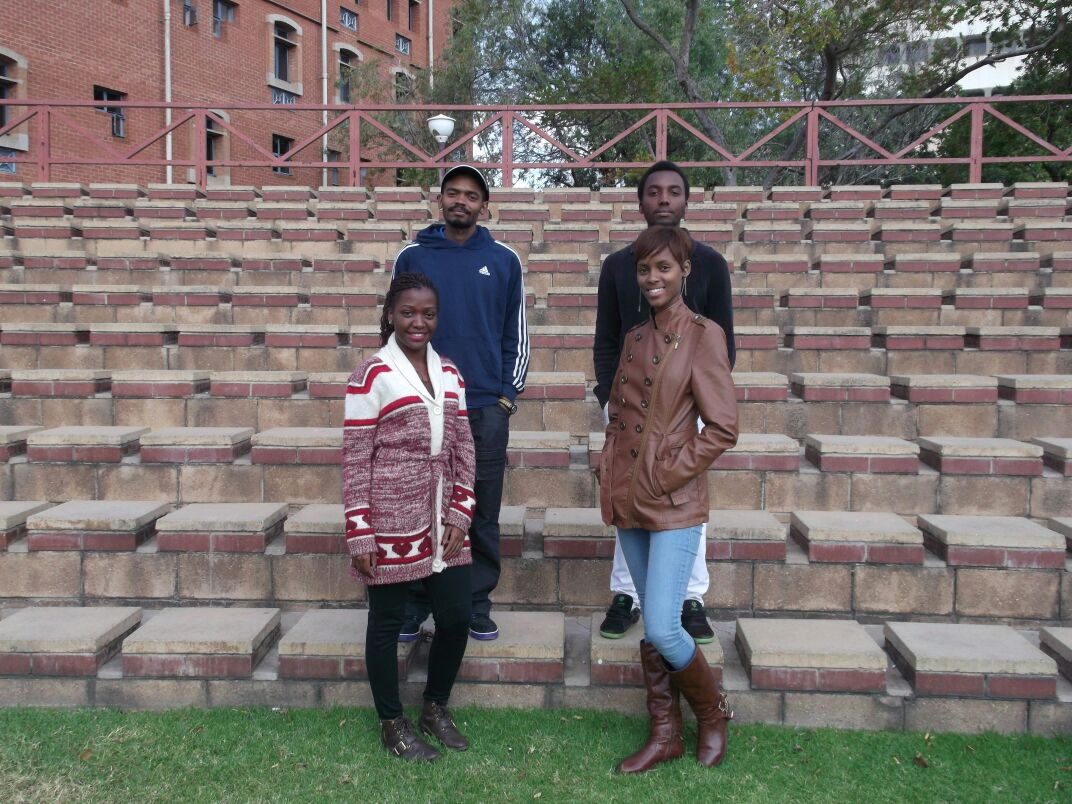
\includegraphics[width=\textwidth]{images/GroupPhoto}

{\large University of Pretoria, Department of Computer Science}\\

{\large 02 May 2016}\\[3cm]

\vfil

\end{titlepage}
\newpage
\tableofcontents
\newpage

\section{The Team}
\subsection{Mpho Baloyi}
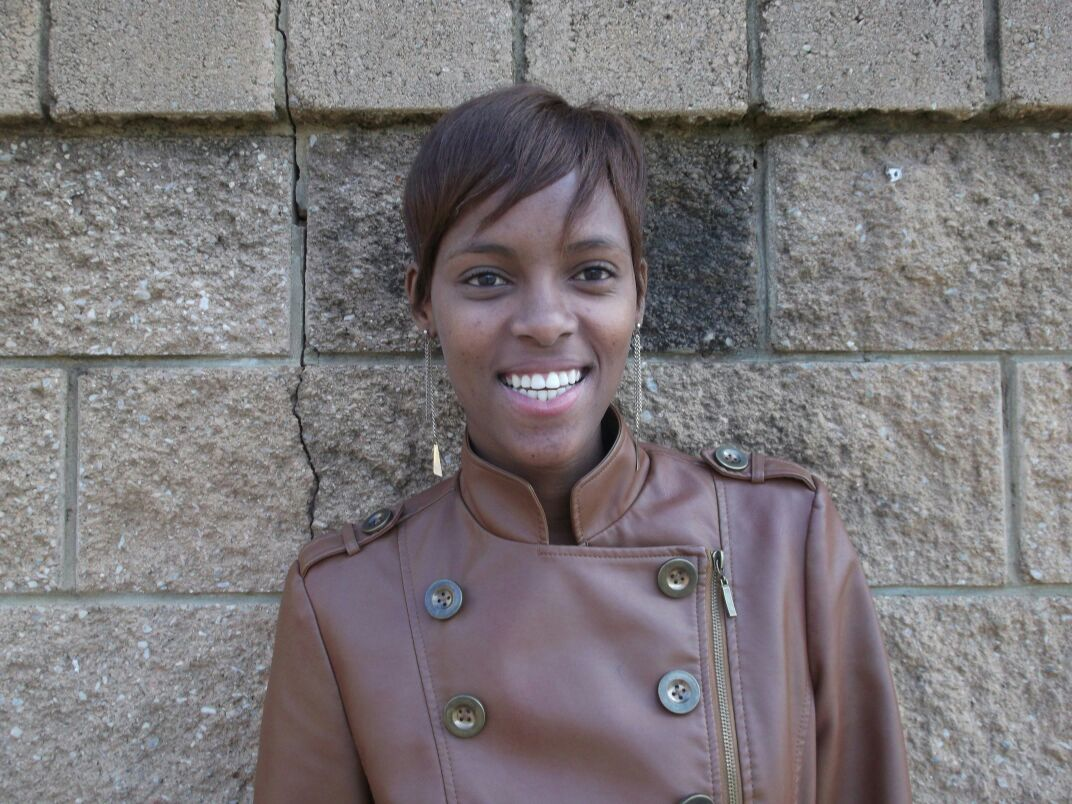
\includegraphics[width=\textwidth]{images/Mpho}
\subsubsection{Interests}
\begin{itemize}
\item Keeping abreast with new technologies
\item Learning and using new technologies to solve problems
\item Reading up and doing research on new and old concepts in computer science
\item Solving riddles and puzzles
\item Helping people through ICT
\end{itemize}
\subsubsection{Technical Skills}
\begin{itemize}
\item Solid programming skills in java,c++ and python
\item Fair amount of knowledge in assembly programming
\item Web development with HTML,JAVASCRIPT,JQUERY,CSS,PHP,AJAX,ANGULARJS
\item Interaction Design
\item Database design with MySQL
\item Understanding of process development
\item Unit testing,mocking and dependency Injection
\end{itemize}
\subsubsection{Non-Technical Strengths}
\begin{itemize}
\item Excellent Communication skills
\item Patient
\item Creative approach to problem solving
\item Pay attention to detail
\item Excellent planning skills
\item Ability to grasp concepts quickly
\item Willingness to learn new things
\item Ability to interpret and follow technical plans
\item Ability to collaborate and work efficiently with other people
\item Ability to work under pressure
\end{itemize}
\subsubsection{Relevant Past Experiences}
Work in the mini-project of the university of Pretoria taught me important skills in software engineering such as unit testing,dependency injection,mocking and working with different technologies. I believe that these skills will be valuable to the development of this project as they apply in every area of software development.
\subsubsection{Reasons for wanting to do the project}
I want to do this project because it provides me with the opportunity to work with different kinds of technologies and devices and to learn new ways of collecting data.
\newpage
\subsection{Hlengekile Jita}
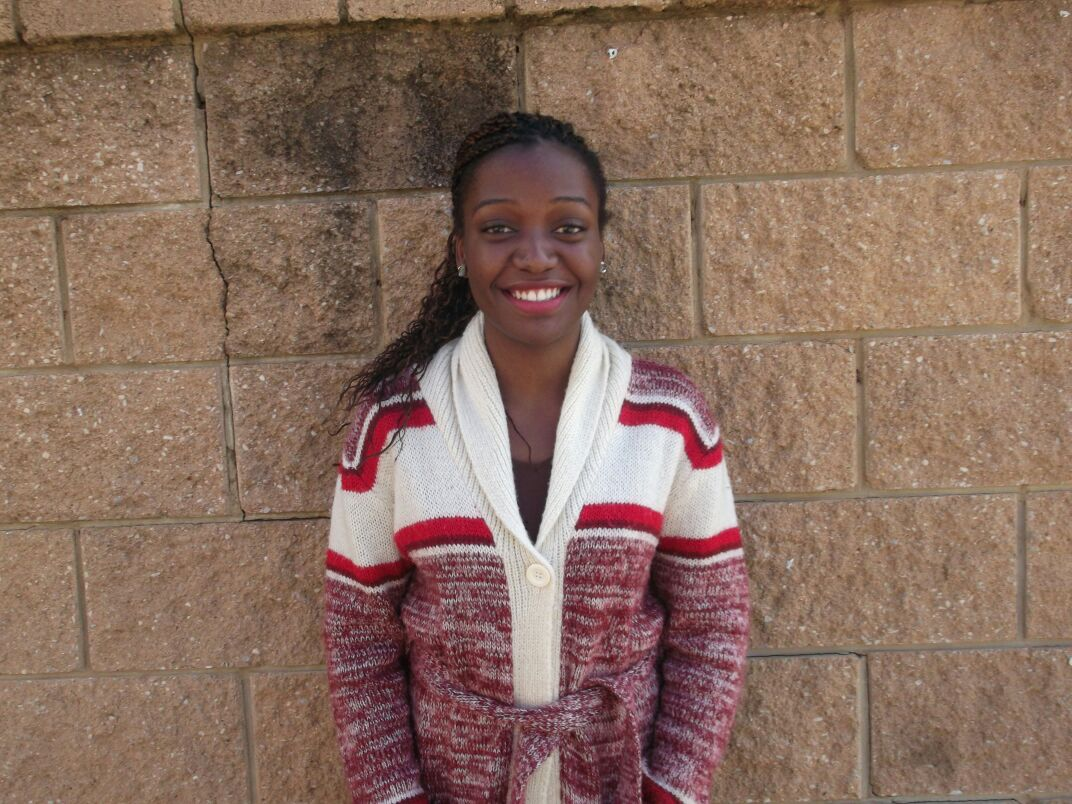
\includegraphics[width=\textwidth]{images/Hlengi}
\subsubsection{Interests}
\begin{itemize}
\item Playing around with gadgets and new technologies
\item Reading up on the role of ICT in communities especially in education
\item Finding out how IT can better business information systems
\end{itemize}
\subsubsection{Technical Skills}
\begin{itemize}
\item Microsoft Office - Word, Excel, Access, PowerPoint
\item Programming - Java, C++, Python, Android
\item Database Design - MySQL
\item Web Development - XHTML, HTML5, CSS, JavaScript, PHP
\end{itemize}
\subsubsection{Non-Technical Strengths}
\begin{itemize}
\item Good leader
\item Excellent communication skills both verbal and written
\item Works well under pressure
\item Great at teamwork
\item Sociable character that gets along with people
\item Organized individual with meticulous planning skills
\item Determined
\end{itemize}
\subsubsection{Relevant Past Experiences}
Some of my past experiences which I  believe will add value to the project is that I have often worked on data processing projects, during my vacation work at the CSIR. Example of this include Twitter data analysis and normalization for text processing. I think that processing information about the networks will be an integral part of this project. I have also got experience working with networks through the module COS 332.
 
In addition to that, my recent experience working on the COS 301 Min-Project has also given me invaluable experience in terms of the software engineering process and working together with people towards the goal of a working software system.
\subsubsection{Reasons for wanting to do the project}
The reason I want to do this project is that I have a great interest in networks and how they work. I think this project will give me great insight into that as well as give me a chance learn about a variety of things such as the EC2 API. I'm also quite excited to create an integrated visualization from which people and more specifically clients of AWS can learn about their networks.
\newpage
\subsection{Moses Mayimela}
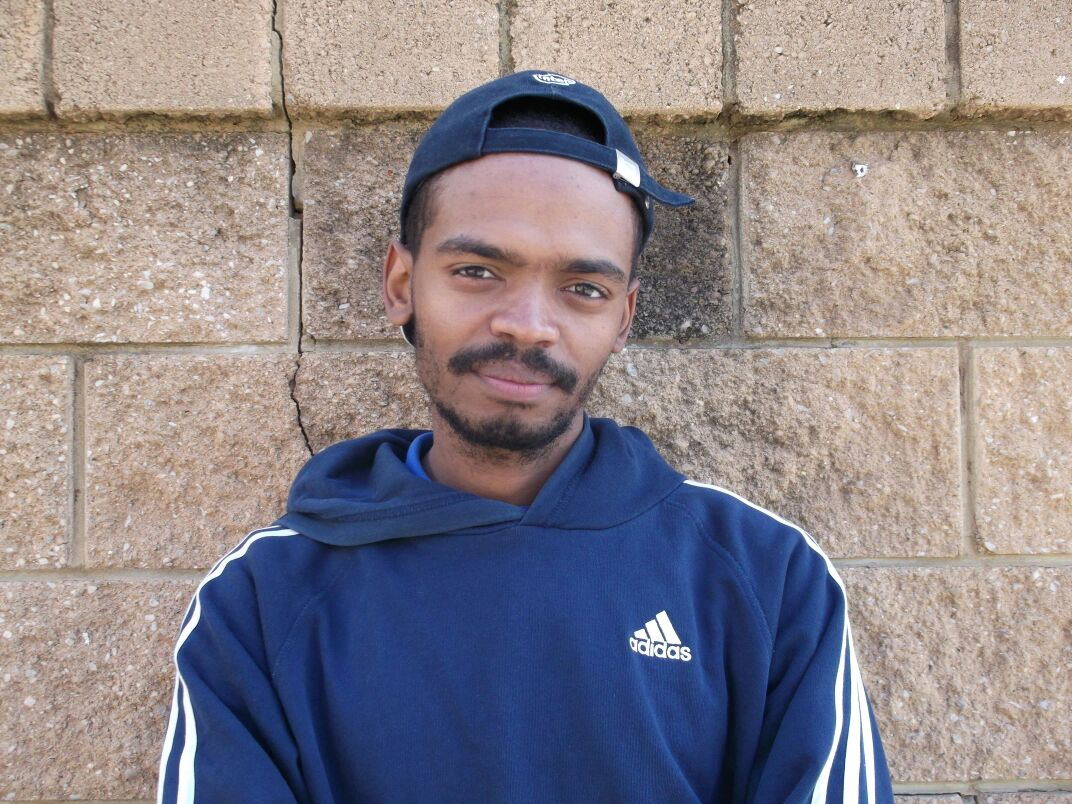
\includegraphics[width=\textwidth]{images/Moses}
\subsubsection{Interests}
\begin{itemize}
\item Keeping up to date with the latest technologies e.g Raspberry pi and Intel Edison.
\item Reading Tech reviews and comparisons on software and hardware systems such as BLE vs Classic Bluetooth.
\item Taking part in hackerthons e.g Hack4Water.
\end{itemize}
\subsubsection{Technical Skills}
\begin{itemize}
\item Programming skills in:
\begin{enumerate}
\item Java.
\item C for embedded Systems (8 bit and 32 bit) and PC applications.
\item C++.
\item C\#.
\item Python.
\end{enumerate}
\item Knowledge in assembly programming for embedded (8 bit and 32 bit) and PC applications.
\item Web development with:\\
HTML,CSS, Javascript, NodeJS (Javascript framework),PHP and AJAX
\item Database design with MySQL,MSSQL and Postgresql.
\item Unit testing,mocking and dependency Injection
\item Familiar with GSM/3G Modules AT commands.
\item Experience with Linux servers.
\end{itemize}
\subsubsection{Non-Technical Strengths}
\begin{itemize}
\item I like working with people who love what they do.
\item I can lead a team and I also respect a leader.
\item I am always willing to learn and expand my horizons.
\item I am open minded to people's opinions.
\end{itemize}
\subsubsection{Relevant Past Experiences}
\begin{itemize}
\item Won, breakthrough developer award for 2015 in the MTN M2M (IoT) competition.\\
http://www.mind2machine.co.za \\
https://www.youtube.com/watch?v=HZlryrw1Ois.
\item 2nd place at the Hack4Water Hackathon in April 2016.\\
https://twitter.com/hashtag/hack4water
\end{itemize}
\subsubsection{Reasons for wanting to do the project}
This project will provide an opportunity for me to expand my knowledge in programming while providing a fully functional solution for the client. The technologies in this project will also help me learn better software standards. Through this project, I can personally learn how I can make myself better and improve my contribution in a way that matters when working with people.
\newpage
\subsection{Themba Mbhele}
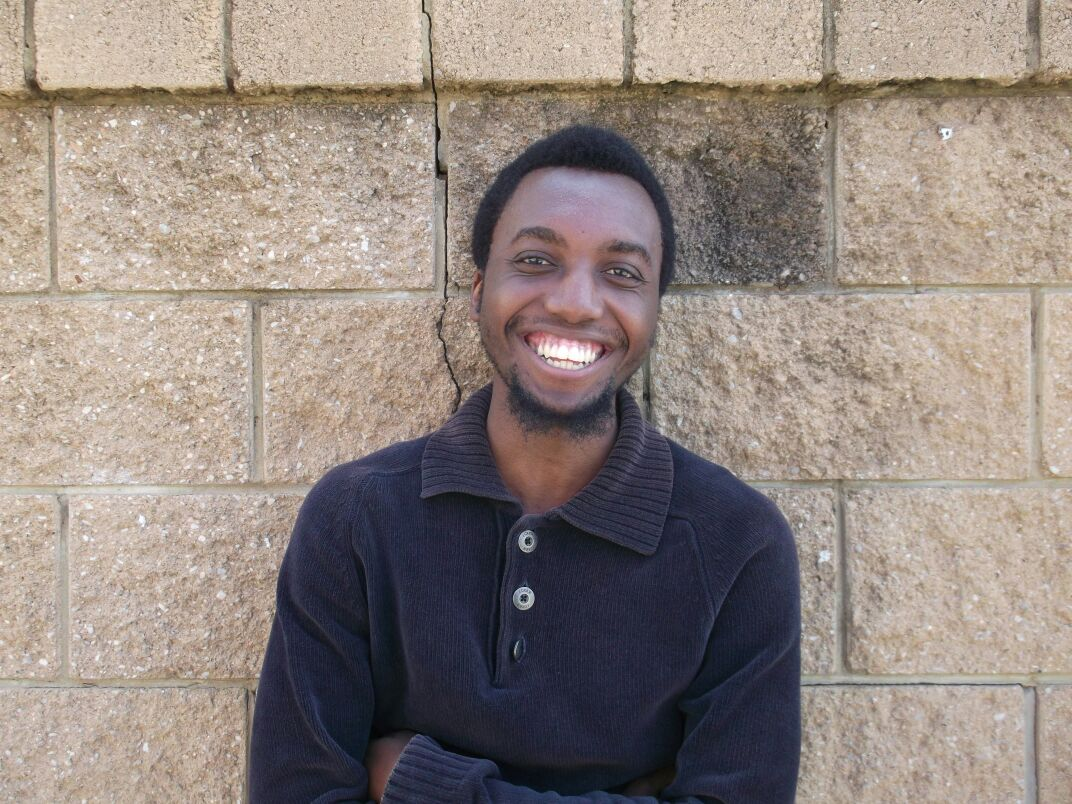
\includegraphics[width=\textwidth]{images/Themba}
\subsubsection{Interests}
\begin{itemize}
    \item Gaming
    \item Artificial Intelligence
    \item Keeping up with the new developments in the Computer Science field
    \item Participating in IT challenges e.g Standard Bank IT Challenge
\end{itemize}
\subsubsection{Technical Skills}
\begin{itemize}
    \item Strong programming skills in C++ and Java
    \item Linux 64-bit assembler knowledge
    \item Unit testing, mocking, and dependency injection
    \item Web Dev - HTML5, CSS, WebGL, JavaScript, PHP
\end{itemize}
\subsubsection{Non-Technical Strengths}
\begin{itemize}
    \item Excellent time management skills
    \item I am a Dedicated student who will put in the necessary effort to make a success of any project that I am a part of.
    \item I am a Team player
\end{itemize}
\subsubsection{Reasons for wanting to do the project}
I want to be a part of this project because I will be exposed to technologies that I have not been exposed to before and because that is an interest of mine, I will have continuous motivation to complete the project.

\section{Project Execution}
\subsection{Project Development Methodology}
\label{Project Design Methodology}
\subsubsection{Data Collection}
The first step is to retrieve the network data. The information may be retrieved from a file or web source.
\subsubsection{Data Classification}
The data will now be validated for correctness. If the data is valid, the different members of the network (parent node, sub-parent node and leaf nodes)
will be identified and classified accordingly. To arrange the data, data structures such as trees will be used.\\
The members of the network that have been identified are:
\begin{itemize}
	\item \textbf{Parent node:} This is the member from which all the other members will be referenced (This is the Main parent or root node).
	\item \textbf{Sub-Parent node:} This is a member that is referenced from another member and has other members that are referenced through it (It is a child with children).
	\item \textbf{Leaf node:} This member is at the lowest level of the tree data structure, it is referenced through a parent and has no members that are referenced through it ( It has no children).
\end{itemize}
\newpage
\subsubsection{Data visualization}
After all the data has been retrieved successfully and the members classified to the respective types, the data will then be loaded to the screen for visual representation (visualize). At this stage, the data can be viewed while allowing interactions for the user. The interactions will include zooming in and out of the visualizer,panning around the graph, click events for more information on a specific member of the network.\\ \\
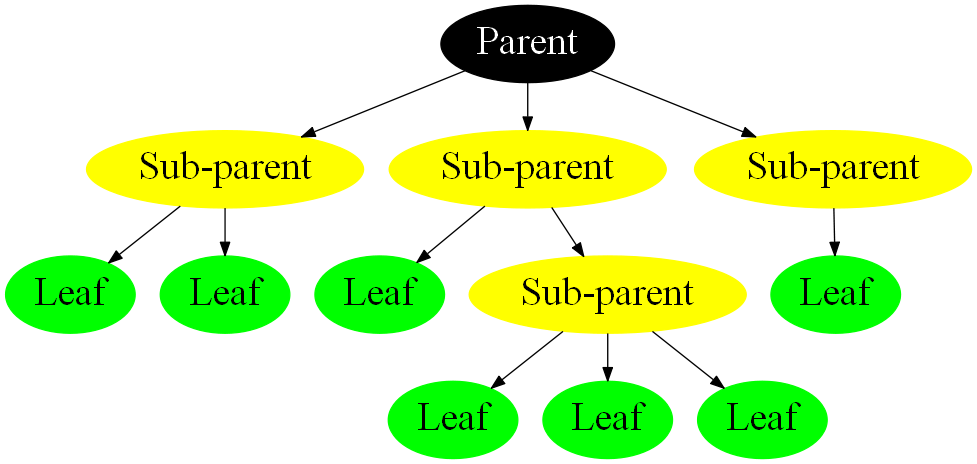
\includegraphics[width=\textwidth]{images/graph1.png}
\begin{center}
Data organization as data structure and basic representation
\end{center}
The image above is a basic representation of how data structures will be used to organize the data and also a starting point as to how the data will be visualized.
\subsection{Communication With Client}
To keep the clients informed we are going to use the following means of communication
\subsubsection{email}
\begin{itemize}
\item To inform the client of our progress
\item To address any issues or concerns that they client may have
\item To acquire information from the client
\item To require any resources that the client has to offer for their project,..
\end{itemize}
\subsubsection{Phone calls}
This will only be used to address very urgent matters if they arise during the course of the project development
however this will only be done with permission from the client and during business hours.
\subsubsection{Regular Meetings}
These will take place depending on the clients availability and willingness.
We may discuss the progress of the project,to address any concerns,etc.
\subsubsection{GIT}
Access to our git repository will be provided to the client,so the client can be able to monitor
our progress and have access to the project material.
We are also open to any means of communication that the client may prefer or suggest.
\subsection{Technical Challenges}
\begin{itemize}
\item Learning the EC2 API 

As this is a very specific technology and one that we have not encountered before but we have a strong believe that 
through more research,more information from the client and our previous experiences with using an API we can overcome this challenge.

\item Retrieving Data from Amazon

This challenge is only due to the lack of information at this stage we plan to overcome this challenge by using either XML or JSON.
\end{itemize}
\subsection{Technologies}
The following technologies will be used for the front-end:
\begin{itemize}
\item HTML5
\item WebGL
\end{itemize}
The following technologies will be used for the back-end:
\begin{itemize}
\item Java
\end{itemize}
\end{document}
